% AA-61
\chapter{Generatory półprostych algebr Liego i relacje Serre'a}
\label{aa:ch:lie-serre-relations}

W AA-59 i AA-60 wyprowadziliśmy z półprostoty rozkład korzeniowy, jednowymiarowość przestrzeni korzeniowych i aksjomaty układu korzeni. Teraz wykorzystamy bazę układu z AA-56, aby opisać generatory algebry i rozkład na ideały proste. Nie zakładamy twierdzenia o prezentacji Serre'a: na razie wyprowadzamy relacje spełniane przez generatory już istniejącej algebry.

W całym rozdziale $K$ jest algebraicznie domkniętym ciałem charakterystyki zero, $\mathfrak g$ niezerową skończenie wymiarową półprostą algebrą Liego nad $K$, $\mathfrak h$ jej maksymalną podalgebrą toralną, a $\Phi$ zbiorem korzeni względem $\mathfrak h$. Korzystamy z realizacji rzeczywistej $\alpha\mapsto\bar\alpha$ z Twierdzenia~\ref{aa:tw:lie-root-realization}. Ponieważ realizacja wykorzystuje współrzędne względem bazy $\mathfrak h$, zachowuje ona wszystkie zależności liniowe o współczynnikach wymiernych. Wybieramy bazę układu rzeczywistego i oznaczamy odpowiadające jej korzenie przez $\Delta=(\alpha_1,\ldots,\alpha_r)$.

\section{Korzenie proste i rozkład trójkątny}

\begin{lemat}
\label{aa:lem:lie-simple-root-basis}
Niech $\mathfrak g$ będzie niezerową skończenie wymiarową półprostą algebrą Liego nad algebraicznie domkniętym ciałem $K$ charakterystyki zero, $\mathfrak h$ jej maksymalną podalgebrą toralną, $\Phi$ zbiorem korzeni, a $\Delta=(\alpha_1,\ldots,\alpha_r)$ bazą układu korzeni w realizacji z Twierdzenia~\ref{aa:tw:lie-root-realization}. Elementy $\alpha_1,\ldots,\alpha_r$ są bazą $\mathfrak h^*$ nad $K$. Elementy $h_i=h_{\alpha_i}$ z Twierdzenia~\ref{aa:tw:root-sl2-triple} tworzą bazę $\mathfrak h$. Każdy korzeń $\beta$ ma jednoznaczny zapis $\beta=\sum_i n_i\alpha_i$, w którym $n_i\in\mathbb Z$ są albo wszystkie nieujemne, albo wszystkie niedodatnie.
\end{lemat}
\begin{proof}
W konstrukcji realizacji z AA-60 wszystkie korzenie mają całkowite współrzędne względem bazy $\mathfrak h$ złożonej z elementów $h_\gamma$. Macierz kolumn odpowiadających $\bar\alpha_i$ jest kwadratowa i ma niezerowy wyznacznik nad $\mathbb R$, ponieważ tworzą one bazę przestrzeni rzeczywistej. Jej wyznacznik jest liczbą całkowitą, więc nie znika również nad $K$. Dowodzi to pierwszej tezy. Izomorfizm $\mathfrak h\to\mathfrak h^*$ zadany przez niezdegenerowaną formę Killinga przekształca $t_{\alpha_i}$ w $\alpha_i$. Zatem $t_{\alpha_i}$ tworzą bazę, podobnie jak ich niezerowe wielokrotności $h_i$. Całkowite współrzędne korzeni o odpowiednich znakach wynikają z Definicji~\ref{aa:def:root-base}; równości między wektorami całkowitymi przenoszą się do $K$. Jednoznaczność wynika z niezależności liniowej.
\end{proof}

\begin{definicja}
\label{aa:def:lie-positive-height}
Dla ustalonej bazy $\Delta$ z Lematu~\ref{aa:lem:lie-simple-root-basis} korzeń $\beta=\sum_i n_i\alpha_i$ nazywamy dodatnim, jeśli wszystkie $n_i\ge0$, i ujemnym, jeśli wszystkie $n_i\le0$. Zbiory takich korzeni oznaczamy przez $\Phi^+,\Phi^-$. Wysokością korzenia $\beta$ nazywamy liczbę całkowitą $\operatorname{ht}(\beta)=\sum_i n_i$. Dla każdego $\beta\in\Phi^+$ wysokość jest dodatnia, gdyż $\beta\ne0$.
\end{definicja}

\begin{lemat}[Odejmowanie korzenia prostego]
\label{aa:lem:lie-root-descent}
Niech $\mathfrak g$ będzie niezerową skończenie wymiarową półprostą algebrą Liego nad algebraicznie domkniętym ciałem $K$ charakterystyki zero, $\mathfrak h$ jej maksymalną podalgebrą toralną, $\Phi$ zbiorem korzeni, a $\Delta=(\alpha_1,\ldots,\alpha_r)$ bazą układu korzeni w realizacji z Twierdzenia~\ref{aa:tw:lie-root-realization}. Jeśli $\beta\in\Phi^+\setminus\Delta$, istnieje $\alpha_i\in\Delta$, dla którego $\beta-\alpha_i\in\Phi^+$ i $\operatorname{ht}(\beta-\alpha_i)=\operatorname{ht}(\beta)-1$.
\end{lemat}
\begin{proof}
Zapiszmy $\beta=\sum_i n_i\alpha_i$. W rzeczywistym modelu
\[
 0<(\bar\beta,\bar\beta)=\sum_i n_i(\bar\beta,\bar\alpha_i).
\]
Istnieje więc $i$ z $n_i>0$ i $(\bar\beta,\bar\alpha_i)>0$. Korzenie $\beta,\alpha_i$ nie są proporcjonalne, bo układ jest zredukowany, a $\beta$ nie jest prosty. Z Twierdzenia~\ref{aa:tw:lie-root-realization} liczba $b=\beta(h_i)$ jest obrazem dodatniej liczby całkowitej w $K$; nierówność dotyczy tej liczby całkowitej, a nie porządku w $K$. W Twierdzeniu~\ref{aa:tw:lie-root-string} mamy $b=p-q>0$, skąd $p\ge1$. Zatem $\beta-\alpha_i$ jest korzeniem; jego współczynniki w bazie są nieujemne, gdyż $n_i>0$. Suma współczynników zmniejsza się o jeden.
\end{proof}

\begin{twierdzenie}[Rozkład trójkątny]
\label{aa:tw:lie-triangular-decomposition}
Niech $\mathfrak g$ będzie niezerową skończenie wymiarową półprostą algebrą Liego nad algebraicznie domkniętym ciałem $K$ charakterystyki zero, $\mathfrak h$ jej maksymalną podalgebrą toralną, $\Phi$ zbiorem korzeni, a $\Delta=(\alpha_1,\ldots,\alpha_r)$ bazą układu korzeni w realizacji z Twierdzenia~\ref{aa:tw:lie-root-realization}. Niech $\mathfrak n^+=\bigoplus_{\alpha\in\Phi^+}\mathfrak g_\alpha$ oraz $\mathfrak n^-=\bigoplus_{\alpha\in\Phi^-}\mathfrak g_\alpha$. Są to nilpotentne podalgebry i
\[
 \mathfrak g=\mathfrak n^-\oplus\mathfrak h\oplus\mathfrak n^+
\]
jako suma prosta przestrzeni liniowych. Podalgebry $\mathfrak b^\pm=\mathfrak h\oplus\mathfrak n^\pm$ są rozwiązalne, a $\mathfrak n^\pm$ są w nich ideałami.
\end{twierdzenie}
\begin{proof}
Nawias przestrzeni o korzeniach $\alpha,\beta$ należy do przestrzeni o korzeniu $\alpha+\beta$ lub znika, jeśli suma nie jest korzeniem i nie jest zerem. Dla dwóch dodatnich korzeni suma, jeśli jest korzeniem, jest dodatnia; analogicznie dla ujemnych. Otrzymujemy podalgebry. Suma prosta wynika z rozkładu korzeniowego.

Z niezerowości $\mathfrak g$ i rozkładu korzeniowego oraz faktu, że korzenie rozpinają $\mathfrak h^*$, wynika $\Phi\ne\varnothing$. Zatem $\Phi^+\ne\varnothing$. Niech $M=\max_{\alpha\in\Phi^+}\operatorname{ht}(\alpha)$. Dla $k\ge1$ połóżmy $N_k=\bigoplus_{\alpha\in\Phi^+,\ \operatorname{ht}(\alpha)\ge k}\mathfrak g_\alpha$. Mamy $[N_i,N_j]\subset N_{i+j}$, ponieważ wysokość jest addytywna. Jeżeli $C^1=\mathfrak n^+$ i $C^{k+1}=[\mathfrak n^+,C^k]$, to indukcyjnie $C^k\subset N_k$. Ponieważ $N_{M+1}=0$, szereg centralny zstępujący kończy się zerem. Dla $\mathfrak n^-$ stosujemy tę samą argumentację do wysokości $-\operatorname{ht}$.

Ponadto $[\mathfrak h,\mathfrak n^\pm]\subset\mathfrak n^\pm$ i $[\mathfrak h,\mathfrak h]=0$. Stąd $\mathfrak b^\pm$ są podalgebrami z ideałami $\mathfrak n^\pm$, a $[\mathfrak b^\pm,\mathfrak b^\pm]\subset\mathfrak n^\pm$. Nilpotentność implikuje rozwiązalność na mocy Lematu~\ref{aa:lem:lie-series}; jeżeli $D^0(\mathfrak l)=\mathfrak l$ oraz $D^{k+1}(\mathfrak l)=[D^k(\mathfrak l),D^k(\mathfrak l)]$, to $D^1(\mathfrak b^\pm)\subset D^0(\mathfrak n^\pm)$, a indukcja daje $D^{k+1}(\mathfrak b^\pm)\subset D^k(\mathfrak n^\pm)$ dla każdego $k\ge0$. Zatem $\mathfrak b^\pm$ są rozwiązalne.
\end{proof}

\begin{center}
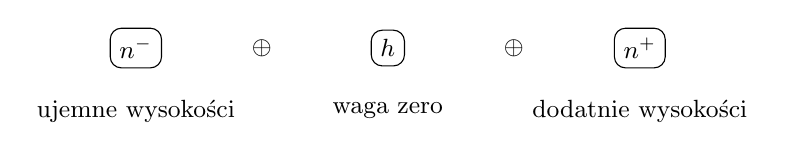
\begin{tikzpicture}[every node/.style={font=\small}]
\node[draw,rounded corners] (m) at (-3.2,0) {$\mathfrak n^-$};
\node[draw,rounded corners] (h) at (0,0) {$\mathfrak h$};
\node[draw,rounded corners] (p) at (3.2,0) {$\mathfrak n^+$};
\node at (-3.2,-.8) {ujemne wysokości};
\node at (0,-.8) {waga zero};
\node at (3.2,-.8) {dodatnie wysokości};
\node at (-1.6,0) {$\oplus$};
\node at (1.6,0) {$\oplus$};
\end{tikzpicture}

\small Rozkład przestrzeni liniowej; składniki nie muszą być ideałami $\mathfrak g$.
\end{center}

\section{Generatory związane z korzeniami prostymi}

Dla każdego $i$ wybieramy $0\ne e_i\in\mathfrak g_{\alpha_i}$ i element $f_i\in\mathfrak g_{-\alpha_i}$ taki, że $[e_i,f_i]=h_i$. Istnienie zapewnia Twierdzenie~\ref{aa:tw:root-sl2-triple}; jednoznaczność $f_i$ wynika z jednowymiarowości przestrzeni i niezerowości nawiasu.

\begin{twierdzenie}
\label{aa:tw:lie-simple-generators}
Niech $\mathfrak g$ będzie niezerową skończenie wymiarową półprostą algebrą Liego nad algebraicznie domkniętym ciałem $K$ charakterystyki zero, $\mathfrak h$ jej maksymalną podalgebrą toralną, $\Phi$ zbiorem korzeni, a $\Delta=(\alpha_1,\ldots,\alpha_r)$ bazą układu korzeni w realizacji z Twierdzenia~\ref{aa:tw:lie-root-realization}. Dla każdego $i$ wybierzmy $0\ne e_i\in\mathfrak g_{\alpha_i}$ i $f_i\in\mathfrak g_{-\alpha_i}$ spełniający $[e_i,f_i]=h_{\alpha_i}$. Podalgebra $\mathfrak n^+$ z Twierdzenia~\ref{aa:tw:lie-triangular-decomposition} jest generowana przez $e_1,\ldots,e_r$, podalgebra $\mathfrak n^-$ przez $f_1,\ldots,f_r$, a $\mathfrak g$ przez wszystkie $e_i,f_i$.
\end{twierdzenie}
\begin{proof}
Niech $\mathfrak u$ będzie podalgebrą generowaną przez $e_i$. Zawiera się w $\mathfrak n^+$. Indukujemy po wysokości dodatniego korzenia $\beta$. Dla wysokości jeden jest on prosty, więc $\mathfrak g_\beta=Ke_i\subset\mathfrak u$. Przy większej wysokości Lemat~\ref{aa:lem:lie-root-descent} daje $\gamma=\beta-\alpha_i\in\Phi^+$ o mniejszej wysokości. Z indukcji $\mathfrak g_\gamma\subset\mathfrak u$. Wniosek~\ref{aa:cor:lie-root-reflection} daje
$[\mathfrak g_{\alpha_i},\mathfrak g_\gamma]=\mathfrak g_\beta$, stąd $\mathfrak g_\beta\subset\mathfrak u$. Otrzymujemy $\mathfrak u=\mathfrak n^+$.
Dla ujemnych korzeni stosujemy ten sam dowód do bazy $-\Delta$ i generatorów $f_i$. Podalgebra generowana przez wszystkie $e_i,f_i$ zawiera także $h_i=[e_i,f_i]$, a więc $\mathfrak h$ na mocy Lematu~\ref{aa:lem:lie-simple-root-basis}. Rozkład trójkątny daje całą $\mathfrak g$.
\end{proof}

\section{Relacje Serre'a}

\begin{twierdzenie}
\label{aa:tw:lie-serre-necessary}
Niech $\mathfrak g$ będzie niezerową skończenie wymiarową półprostą algebrą Liego nad algebraicznie domkniętym ciałem $K$ charakterystyki zero, $\mathfrak h$ jej maksymalną podalgebrą toralną, $\Phi$ zbiorem korzeni, a $\Delta=(\alpha_1,\ldots,\alpha_r)$ bazą układu korzeni w realizacji z Twierdzenia~\ref{aa:tw:lie-root-realization}. Niech $h_i=h_{\alpha_i}$, $0\ne e_i\in\mathfrak g_{\alpha_i}$, $f_i\in\mathfrak g_{-\alpha_i}$ i $[e_i,f_i]=h_i$. Niech $a_{ij}=\alpha_j(h_i)$ dla $1\le i,j\le r$. Generatory $e_i,f_i,h_i$ spełniają relacje
\[
\begin{aligned}
 [h_i,h_j]&=0, &
 [h_i,e_j]&=a_{ij}e_j,\\
 [h_i,f_j]&=-a_{ij}f_j, &
 [e_i,f_j]&=\delta_{ij}h_i.
\end{aligned}
\]
Ponadto dla $i\ne j$ zachodzą relacje Serre'a
\[
 (\operatorname{ad}_{e_i})^{1-a_{ij}}e_j=0,\qquad
 (\operatorname{ad}_{f_i})^{1-a_{ij}}f_j=0.
\]
W obu relacjach potęga $-a_{ij}$ zamiast $1-a_{ij}$ daje wektor niezerowy.
\end{twierdzenie}
\begin{proof}
Macierz $(a_{ij})$ jest macierzą Cartana w konwencji AA-56, ponieważ $a_{ij}=2(\bar\alpha_i,\bar\alpha_j)/(\bar\alpha_i,\bar\alpha_i)$. W szczególności $a_{ii}=2$, a dla $i\ne j$ mamy $a_{ij}\le0$. Abelowość $\mathfrak h$, definicje przestrzeni korzeniowych i normalizacja trójek dają pierwsze trzy relacje i $[e_i,f_i]=h_i$. Jeśli $i\ne j$, różnica $\alpha_i-\alpha_j$ nie jest korzeniem, gdyż ma współczynniki o różnych znakach w bazie. Nie jest również zerem. Reguła nawiasów daje więc $[e_i,f_j]=0$.

W ciągu korzeniowym przez $\alpha_j$ w kierunku $\alpha_i$ nie ma korzenia $\alpha_j-\alpha_i$, więc $p=0$. Twierdzenie~\ref{aa:tw:lie-root-string} daje $a_{ij}=p-q=-q$. Występują dokładnie korzenie $\alpha_j+k\alpha_i$ dla $0\le k\le -a_{ij}$. Działanie $\operatorname{ad}_{e_i}$ na kolejnych przestrzeniach jest niezerowe i surjektywne poza ostatnią, a na ostatniej znika, bo następna waga nie występuje. Indukcja pokazuje, że $(\operatorname{ad}_{e_i})^k e_j\ne0$ dla $0\le k\le -a_{ij}$, zaś dla $k=1-a_{ij}$ dostajemy zero. Stosując ten argument do bazy $-\Delta$, której macierz Cartana jest taka sama, oraz trójek $(f_i,e_i,-h_i)$, otrzymujemy drugą relację i niezerowość poprzedniej potęgi.
\end{proof}

\begin{uwaga}
Relacje te są na razie warunkami koniecznymi. Jeśli skonstruujemy abstrakcyjną algebrę Liego z generatorami i dokładnie tymi relacjami, Twierdzenie~\ref{aa:tw:lie-simple-generators} zapewni surjektywny homomorfizm na $\mathfrak g$. Wykazanie jego iniektywności i istnienia odpowiedniej algebry dla każdej macierzy Cartana typu skończonego wymaga dalszych argumentów.
\end{uwaga}

\section{Ideały i składowe układu korzeni}

\begin{lemat}
\label{aa:lem:lie-ideal-weight-components}
Niech $\mathfrak g$ będzie skończenie wymiarową półprostą algebrą Liego nad algebraicznie domkniętym ciałem $K$ charakterystyki zero, $\mathfrak h$ jej maksymalną podalgebrą toralną, a $\Phi$ zbiorem korzeni. Jeżeli $\mathfrak a$ jest ideałem $\mathfrak g$, to
\[
 \mathfrak a=(\mathfrak a\cap\mathfrak h)\oplus
 \bigoplus_{\alpha\in\Phi}(\mathfrak a\cap\mathfrak g_\alpha).
\]
\end{lemat}
\begin{proof}
Wybieramy $t\in\mathfrak h$, dla którego wartości $\lambda(t)$ dla $\lambda\in\Phi\cup\{0\}$ są parami różne. Jest to możliwe: zbiór niedozwolony jest sumą mnogościową skończenie wielu jąder niezerowych funkcjonałów $\lambda-\mu$. Iloczyn ich równań liniowych jest niezerowym wielomianem, który nad nieskończonym ciałem nie może znikać wszędzie. Operator $\operatorname{ad}_t$ ma więc przestrzenie własne dokładnie równe składowym rozkładu korzeniowego. Ideał $\mathfrak a$ jest niezmienniczy względem tego operatora, a zatem względem każdej projekcji wielomianowej
\[
 P_\lambda=\prod_{\mu\in\Phi\cup\{0\},\ \mu\ne\lambda}
 \frac{\operatorname{ad}_t-\mu(t)I}{\lambda(t)-\mu(t)}.
\]
Na przestrzeni wagi $\lambda$ projekcja jest identycznością, a na pozostałych jest zerem. Składowe każdego elementu $\mathfrak a$ należą więc do $\mathfrak a$; odwrotna inkluzja wynika z liniowości ideału.
\end{proof}

\begin{twierdzenie}[Składowe proste]
\label{aa:tw:lie-dynkin-components}
Niech $\mathfrak g$ będzie niezerową skończenie wymiarową półprostą algebrą Liego nad algebraicznie domkniętym ciałem $K$ charakterystyki zero, $\mathfrak h$ jej maksymalną podalgebrą toralną, $\Phi$ zbiorem korzeni, a $\Delta=(\alpha_1,\ldots,\alpha_r)$ bazą układu korzeni w realizacji z Twierdzenia~\ref{aa:tw:lie-root-realization}. Niech $h_i=h_{\alpha_i}$, a $I_1,\ldots,I_s$ będą zbiorami indeksów składowych spójnych diagramu Dynkina bazy $\Delta$. Niech $\Phi_\ell$ będzie zbiorem korzeni, których współczynniki poza $I_\ell$ są zerowe, a $\mathfrak h_\ell=\operatorname{span}_K\{h_i:i\in I_\ell\}$. Wówczas
\[
 \mathfrak g_\ell=\mathfrak h_\ell\oplus
 \bigoplus_{\alpha\in\Phi_\ell}\mathfrak g_\alpha
\]
są niezerowymi prostymi ideałami, komutującymi parami, oraz $\mathfrak g=\bigoplus_{\ell=1}^s\mathfrak g_\ell$. W szczególności $\mathfrak g$ jest prosta wtedy i tylko wtedy, gdy jej układ korzeni jest nierozkładalny.
\end{twierdzenie}
\begin{proof}
Z dowodu Twierdzenia~\ref{aa:tw:root-cartan} korzenie należą do dokładnie jednej z przestrzeni rozpiętych przez proste korzenie poszczególnych składowych. Przestrzenie te są wzajemnie ortogonalne w modelu rzeczywistym. Zatem $\Phi$ jest rozłączną sumą $\Phi_\ell$, a Lemat~\ref{aa:lem:lie-simple-root-basis} daje $\mathfrak h=\bigoplus_\ell\mathfrak h_\ell$. Stąd rozkład $\mathfrak g$ na podprzestrzenie $\mathfrak g_\ell$ jest prosty.

Dla $\alpha\in\Phi_\ell$, $\beta\in\Phi_k$, $k\ne\ell$, suma $\alpha+\beta$ nie może być korzeniem: miałaby niezerowe składowe w dwóch różnych częściach bazy. Nie może też być zerem. Zatem $[\mathfrak g_\alpha,\mathfrak g_\beta]=0$. Ponadto $\beta(h_i)=0$ dla $i\in I_\ell$ dzięki ortogonalności, więc $[\mathfrak h_\ell,\mathfrak g_\beta]=0$. Abelowość $\mathfrak h$ daje komutowanie różnych $\mathfrak g_\ell$.

Sprawdzimy zamknięcie każdej $\mathfrak g_\ell$ na nawias. Dla korzeni z tej samej części ich suma, jeśli jest niezerowym korzeniem, należy do tej części. Jeśli suma jest zerem, wzór z dowodu Twierdzenia~\ref{aa:tw:root-sl2-triple} daje $[x,y]=\kappa(x,y)t_\alpha$ dla $x\in\mathfrak g_\alpha$, $y\in\mathfrak g_{-\alpha}$. Ponieważ $\alpha=\sum_{i\in I_\ell}n_i\alpha_i$, liniowość izomorfizmu wyznaczonego przez formę Killinga daje $t_\alpha=\sum_{i\in I_\ell}n_i t_{\alpha_i}\in\mathfrak h_\ell$. Nawiasy z $\mathfrak h_\ell$ zachowują przestrzenie korzeniowe, a sama $\mathfrak h_\ell$ jest abelowa. To dowodzi zamknięcia. Wraz z komutowaniem innych składników oznacza to, że $\mathfrak g_\ell$ jest ideałem. Nie jest abelowy, gdyż dla $i\in I_\ell$ zawiera trójkę z $[e_i,f_i]=h_i\ne0$.

Niech $\mathfrak a\ne0$ będzie ideałem $\mathfrak g_\ell$. Dzięki komutowaniu pozostałych składników jest ideałem $\mathfrak g$. Z Lematu~\ref{aa:lem:lie-ideal-weight-components} albo zawiera niezerowy element pewnej przestrzeni korzeniowej, albo jest zawarty w $\mathfrak h_\ell$. W drugim przypadku wybierzmy $0\ne t\in\mathfrak a$. Korzenie rozpinają $\mathfrak h^*$, więc istnieje $\beta$ z $\beta(t)\ne0$; ortogonalność części pokazuje, że $\beta\in\Phi_\ell$. Dla $0\ne x\in\mathfrak g_\beta$ mamy $[t,x]=\beta(t)x\in\mathfrak a$, zatem w obu przypadkach $\mathfrak a$ zawiera całą pewną przestrzeń korzeniową, bo jest jednowymiarowa.

Jeżeli zawarta przestrzeń odpowiada korzeniowi ujemnemu, wybieramy $0\ne x\in\mathfrak g_\beta\subset\mathfrak a$ i $y\in\mathfrak g_{-\beta}$ z $\kappa(x,y)\ne0$, korzystając z niezdegenerowanego parowania. Wtedy $[x,y]=\kappa(x,y)t_\beta\in\mathfrak a$, więc $h_\beta\in\mathfrak a$. Ponieważ $[h_\beta,y]=-2y$, cała prosta $\mathfrak g_{-\beta}$ należy do $\mathfrak a$. Możemy więc zacząć od dodatniego korzenia $\beta$. Jeśli $\beta$ nie jest prosty, Lemat~\ref{aa:lem:lie-root-descent} daje $\beta-\alpha_i\in\Phi^+$; z Wniosku~\ref{aa:cor:lie-root-reflection} nawias $[\mathfrak g_\beta,\mathfrak g_{-\alpha_i}]$ jest całą przestrzenią $\mathfrak g_{\beta-\alpha_i}$, zawartą w $\mathfrak a$. Po skończonej liczbie kroków otrzymujemy $e_i\in\mathfrak a$ dla pewnego $i\in I_\ell$. Wtedy $h_i=[e_i,f_i]\in\mathfrak a$ i $[h_i,f_i]=-2f_i$ daje $f_i\in\mathfrak a$.

Jeśli $i,j$ są sąsiednimi wierzchołkami diagramu, to $a_{ij}\ne0$. Nawiasy $[h_i,e_j]=a_{ij}e_j$ i $[h_i,f_j]=-a_{ij}f_j$ dają $e_j,f_j\in\mathfrak a$, a ich nawias daje $h_j$. Spójność pozwala przejść do wszystkich indeksów $I_\ell$. Dowód Twierdzenia~\ref{aa:tw:lie-simple-generators} zastosowany do korzeni tej części (odejmowanie prostego korzenia nie wychodzi poza część) daje wszystkie jej przestrzenie korzeniowe. Stąd $\mathfrak a=\mathfrak g_\ell$. Ostatnia teza wynika z równoważności spójności diagramu i nierozkładalności układu z AA-56.
\end{proof}

\section{Przykład typu A}
\begin{przyklad}
\label{aa:prz:lie-serre-sl3}
Dla $\mathfrak{sl}_3(K)$ wybieramy $\alpha_1=\alpha_{12}$, $\alpha_2=\alpha_{23}$ z Przykładu~\ref{aa:prz:sl3-root-decomposition}. Generatory to
$e_1=E_{12}$, $e_2=E_{23}$, $f_1=E_{21}$, $f_2=E_{32}$ i $h_1=E_{11}-E_{22}$, $h_2=E_{22}-E_{33}$. Macierz Cartana jest równa
$\left(\begin{smallmatrix}2&-1\\-1&2\end{smallmatrix}\right)$.
Dodatnia podalgebra składa się z macierzy ściśle górnotrójkątnych, ujemna z macierzy ściśle dolnotrójkątnych, a $\mathfrak h$ z macierzy diagonalnych o śladzie zero. Z wzoru $E_{ij}E_{kl}=\delta_{jk}E_{il}$ mamy
\[
 [e_1,e_2]=E_{13},\quad [f_1,f_2]=-E_{31},\quad
 [e_1,E_{13}]=[e_2,E_{13}]=0.
\]
Analogicznie $[f_1,E_{31}]=[f_2,E_{31}]=0$. Relacje Serre'a mają zatem wykładnik dwa i nie można go zmniejszyć do jednego. Dodatnia i ujemna podalgebra mają klasę nilpotentności dwa, gdyż ich nawiasy rozpinają odpowiednio $KE_{13}$ i $KE_{31}$, a te przestrzenie komutują ze swoimi podalgebrami. Diagram $A_2$ jest spójny, więc Twierdzenie~\ref{aa:tw:lie-dynkin-components} daje prostotę $\mathfrak{sl}_3(K)$.
\end{przyklad}

Rozdział przygotowuje dowód twierdzenia o prezentacji Serre'a: znamy generatory i wszystkie wskazane relacje w istniejącej algebrze, lecz nie wykazaliśmy jeszcze, że relacje te wyczerpują zależności między generatorami.
